\begin{comment}
\documentclass[10pt]{article}
\usepackage{fullpage, graphicx, url}
\setlength{\parskip}{1ex}
\setlength{\parindent}{0ex}
\title{wguide2}
\begin{document}


\begin{tabular}{ccc}
The Alternative Csound Reference Manual & & \\
Previous & &Next

\end{tabular}

%\hline 
\end{comment}
\section{wguide2}
wguide2�--� A model of beaten plate consisting of two parallel delay-lines and two first-order lowpass filters. \subsection*{Description}


  A model of beaten plate consisting of two parallel delay-lines and two first-order lowpass filters. 
\subsection*{Syntax}


 ar \textbf{wguide2}
 asig, xfreq1, xfreq2, kcutoff1, kcutoff2, kfeedback1, kfeedback2
\subsection*{Performance}


 \emph{asig}
 -- the input of excitation noise 


 \emph{xfreq1, xfreq2}
 -- the frequency (i.e. the inverse of delay time) Changed to x-rate in Csound version 3.59. 


 \emph{kcutoff1, kcutoff2}
 -- the filter cutoff frequency in Hz. 


 \emph{kfeedback1, kfeedback2}
 -- the feedback factor 


 \emph{wguide2}
 is a model of beaten plate consisting of two parallel delay-lines and two first-order lowpass filters. The two feedback lines are mixed and sent to the delay again each cycle. 


  Implementing waveguide algorithms as opcodes, instead of orc instruments, allows the user to set \emph{kr}
 different than \emph{sr}
, allowing better performance particulary when using real-time. 


 


 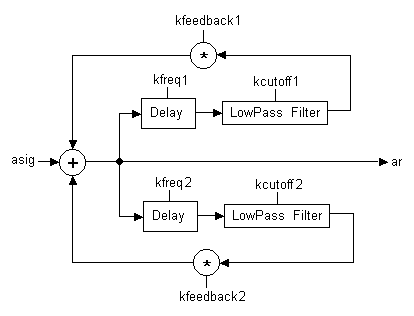
\includegraphics[scale=1]{wguide2} 


 wguide2.
\subsection*{See Also}


 \emph{wguide1}

\subsection*{Credits}


 


 


\begin{tabular}{ccc}
Author: Gabriel Maldonado &Italy &October 1998

\end{tabular}



 


 New in Csound version 3.49
%\hline 


\begin{comment}
\begin{tabular}{lcr}
Previous &Home &Next \\
wguide1 &Up &wrap

\end{tabular}


\end{document}
\end{comment}
